%! Author = borisdeletic
%! Date = 11/05/2023

% Preamble
\documentclass[11pt]{article}

% Document
\begin{document}

\section{Numerical Results}\label{sec:numerical_results}
    The CHMC for nested sampling algorithm was implemented as an optimised C++ library in order to run large scale,
    high dimensional tests.
    We provide a novel application of nested sampling to $\phi^4$-theory to perform experiments.
    The $\phi^4$ action was given as the likelihood function as defined in section~\ref{subsec:nested-sampling-phi4}.

    All input parameter values are listed in appendix~\ref{sec:param_table} and full details about the implementation
    can be found in appendix~\ref{sec:code_implementation}.
    All results were gathered using a single core on the CSD3 compute cluster.

\subsection{Phase Transitions}\label{subsec:phase_transition}
    To investigate the phase transition in $\phi^4$-theory, we aim to measure the mean magnetisation~\eqref{eq:magnetization}
    of the field for a wide range of $\kappa$ \& $\lambda$ values.

    We use a $32 \times 32$ lattice ($D=1024$) and set $n_{\text{live}}=500$ with precision criteria $p=0.1$.
    For this setup, the average number of nested sampling iterations to converge is $i_{\max} \approx 15,000$.

    The mean magnetisation is calculated as the mean value of absolute field value.
    We show the distribution of $\phi(x)$ for an action in the disordered phase in~\cref{fig:magnetisation}.
\begin{figure}[h!]
    \center
    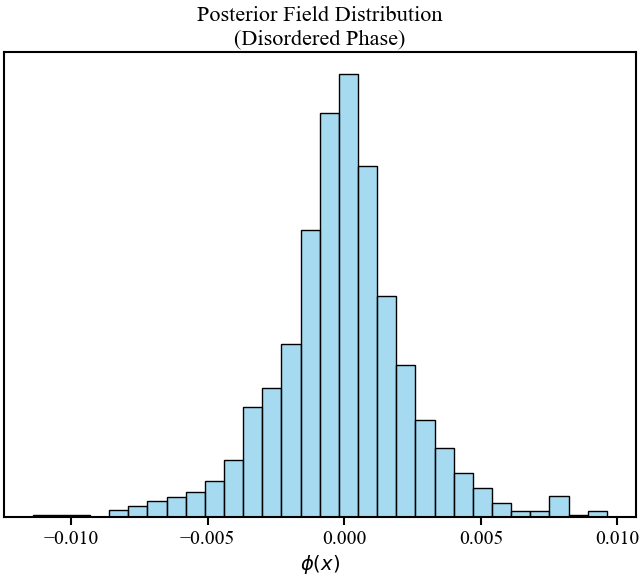
\includegraphics[width=\linewidth]{../figures/Magnetisation}
    \caption{
        The posterior distribution of $\phi(x)$ for an action in the disordered phase.
        For $\kappa = 0.1, \lambda = 0.02$, the distribution is unimodal with narrow variance as it is disordered.
        The magnetisation is the mean of the absolute field value, where $\langle M \rangle \approx 0$ in the above
        action.
    }\label{fig:magnetisation}
    \end{figure}

    We vary the action~\eqref{eq:phi4_action} across the range $\kappa \in (0, 0.3), \lambda \in (0, 0.03)$ for
    a total of $1,000$ unique actions, and calculate $\langle M \rangle$ for each one~\cite{anesthetic}, to construct a phase diagram
    shown in~\cref{fig:phase_diagram}.

    \begin{figure}[h!]
        \center
        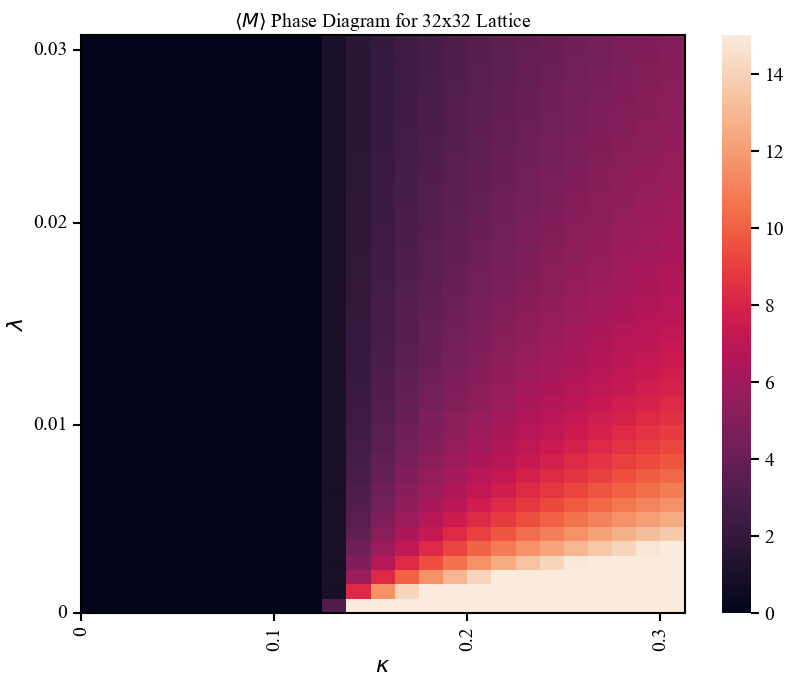
\includegraphics[width=\linewidth]{../figures/PhaseDiagram}
        \caption{
            $\kappa$ vs $\lambda$ phase diagram for 32x32 lattice $\phi^4$-theory.
            For $\kappa \lesssim 0.125$, we see the expression of the disordered phase with $\langle M \rangle = 0$.
            The second-order phase transition is apparent along this boundary, as $\langle M \rangle$ grows suddenly
            across it. \\
            In the ordered phase ($\kappa \gtrsim 0.125$), the mean magnetisation is strongly dependent on the field
            coupling $\lambda$.
            With a weak coupling, the kinetic energy dominates and the field seperates, leading to
            large $\langle M \rangle$.
            We also note that $\lambda$ has a minor influence on the exact critical point in $\kappa$, with the
            critical line having a slight negative slope.
        }\label{fig:phase_diagram}
    \end{figure}

    This phase diagram accurately reconstructs the theoretical result and is verified against other
    simulations~\cite{Pawlowski_2020}.

\subsection{Correlation Functions}\label{subsec:correlation_function}
    The two-point correlation functions are a key quantity related to physical
    observables of the quantum field theory.
    For example, the renormalised mass parameter and correlation length can both be measured with correlation
    functions~\cite{maas2020lattice, brower2018lattice}.

    In the context of a Euclidean $\phi^4$ theory, we define the spatial (equal-time) correlation functions as
    \begin{equation}\label{eq:full_correlation_function}
    C(x_1, x_2) = \langle \phi(x_1) \phi(x_2) \rangle,
    \end{equation}
    where $\langle . \rangle$ denotes the Markov-Chain ensemble average~\eqref{eq:mcmc_observable}.

    Exploiting the translational and rotational symmetry of the $\phi^4$ action, we can fully characterise the two-point
    correlation function in terms of the distance between two points $r$
    \begin{equation}\label{eq:correlation_function}
    C(r) = \langle \phi(x) \phi(x + r) \rangle,
    \end{equation}
    where we now also average over all lattice points $x$.

    Directly calculating correlation functions numerically is prohibitively expensive, requiring $\mathcal{O}(N^3)$
    operations for each microstate.
    Therefore, we use a method of fourier transform and convolution theorem to speed up
    calculation~\cite{Ruge_1994}.

    In the continuous limit $N \rightarrow \infty$ we can write the correlation function for a single microstate at
    Markov-Chain iteration $i$ as
    \begin{equation}\label{eq:continuous_correlation}
        C_{i}(r) = \int_{-\infty}^{\infty} \phi(x) \phi(x + r) dx.
    \end{equation}

    Applying the convolution theorem gives
    \begin{equation}\label{eq:convolution_theorem}
        C_{i}(r) = \mathcal{F}^{-1} \{ |\tilde{\phi}(k)|^2 \}
    \end{equation}
    providing a new way to evaluate the correlation function.
    Using a discrete fast fourier transform, we can therefore calculate the correlation function in
    $\mathcal{O}(N^2 \log N)$.

    Just below the critical point, the correlation function decays exponentially as $C(r) \sim \exp(-r / \xi)$,
    where $\xi$ is defined as the correlation length.
    As we approach the critical point, the correlation length diverges and becomes infinite in the ordered phase.

    We measure the correlation functions on a $128 \times 128$ lattice ($D=16,384$) to minimise finite-size effects.
    Using $n_{\text{live}}=1000$ with fixed $\lambda=0.03$, we show the measured correlation functions for different $\kappa$
    in~\cref{fig:correlation_functions_128}.

    \begin{figure}[h!]
        \center
        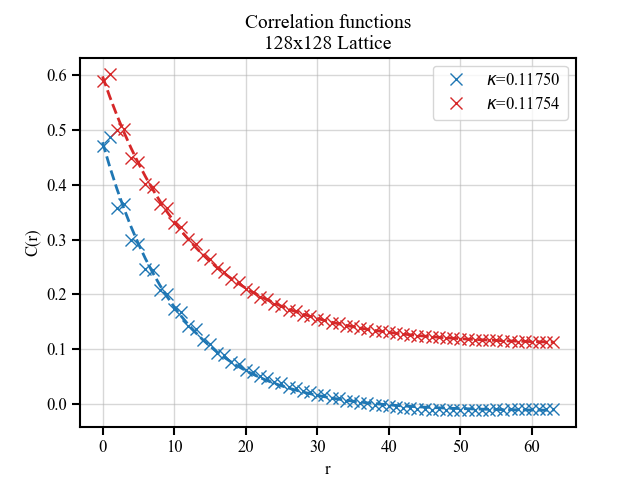
\includegraphics[width=\linewidth]{../figures/CorrelationFunction128}
        \caption{
            Correlation functions for $128 \times 128$ lattice in $\phi^4$-theory for ordered phase (red) and disordered
            phase (blue).
            The fitted exponentials show the expected decay characteristic for both correlation functions.
            In the ordered phase, the correlation function does not decay to 0, but instead shows there is a mean
            magnetisation throughout the field.
        }\label{fig:correlation_functions_128}
    \end{figure}

    We can estimate the correlation length $\xi$ for each value of $\kappa$, and plot the results
    in~\cref{fig:correlation_length} to visualise the phase transition as a divergence in $\xi$.

    \begin{figure}[h!]
        \center
        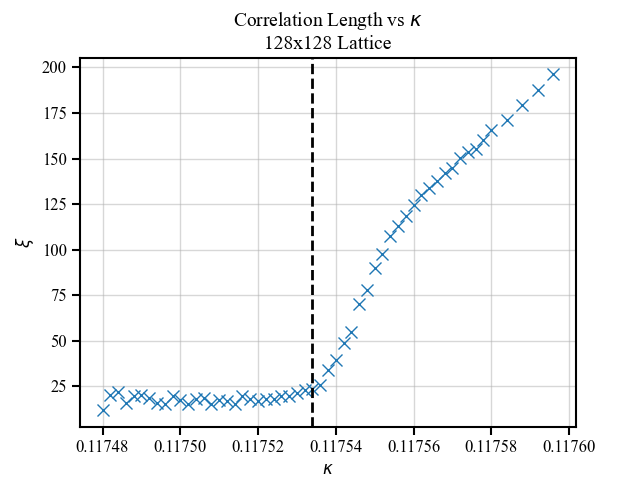
\includegraphics[width=\linewidth]{../figures/CorrelationLength}
        \caption{
            Correlation length ($\xi$) vs $\kappa$ shows the second-order phase transition as the correlation length
            diverges.
            In the disordered phase the correlation length is 0, then begins to increase until it
            exceeds the size of the physical lattice, which marks the ordered phase.
        }\label{fig:correlation_length}
    \end{figure}

    We also calculate the correlation function for a larger lattice of size $512 \times 512$ ($D=262,144$), shown
    in~\cref{fig:correlation_func_512}.
    The phase transition for such a large lattice is very sharp, with the change between ordered and disordered phase
    occurring over $\Delta \kappa \approx 2 \times 10^{-6}$, which our algorithm correctly identifies.

    For the correlation functions on this lattice, there is unexpected cyclic behaviour in the decay.
    We are not sure as to the cause of this phenomenon and further work is required to full understand it.
    \begin{figure}[h!]
        \center
        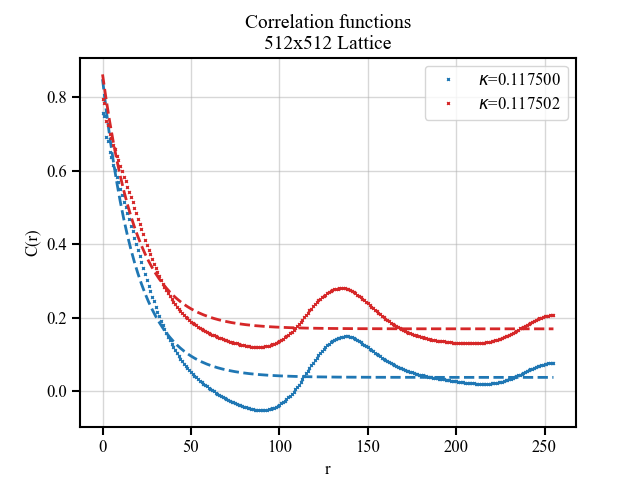
\includegraphics[width=\linewidth]{../figures/CorrelationFunction512}
        \caption{
            Correlation functions for $512 \times 512$ lattice for ordered phase (red) and disordered
            phase (blue).
            Note the phase transition is very sharp, occuring over a range $\Delta \kappa \approx 2 \times 10^{-6}$.
            The correlation functions exhibit cyclic behaviour in decay, which is unexpected and the
            cause is not well understood.
            The calculation of these results demonstrate it is possible to perform nested sampling in dimensions much
            larger ($D=262,144$) than explored previously.
        }\label{fig:correlation_func_512}
    \end{figure}

    The numerical results clearly demonstrate that Constrained HMC with nested sampling is a viable tool for
    lattice field theory.
    The algorithm successfully samples and estimates observables accurately at the critical point, without any
    modifications or difficulty.
    This confirms that leveraging nested sampling for lattice field theory provides strong resistance to topological freezing.


\end{document}
